\documentclass[aspectratio=169]{beamer}
\input{../../../latex/common/preamble}
\graphicspath{{figures/}}
\title{De la donnée capteur à la décision opérationnelle}
\subtitle{Séquence 9 -- Construire des indicateurs sous Excel}
\author{École de l'air et de l'espace}
\date{}

\begin{document}

\begin{frame}
  \titlepage
\end{frame}

\begin{frame}{Bienvenue dans la séquence 9}
  \begin{block}{L'idée qui traverse toute la séance}
    Excel calcule exactement ce qu'on lui demande -- jamais ce qu'on voulait dire. Une formule peut être arithmétiquement parfaite et pourtant totalement dépourvue de sens, si la question posée mélange ce qui ne devrait pas l'être.
  \end{block}
  \begin{itemize}
    \item Le matin, nous construirons des indicateurs corrects avec des tableaux croisés dynamiques (TCD), en apprenant d'abord à repérer ce qu'un calcul mal posé peut cacher.
    \item L'après-midi, nous chercherons un seuil propre à chaque type d'installation avec RECHERCHEX, plutôt que d'appliquer partout le même seuil pédagogique.
    \item La question n'est jamais « la formule est-elle juste ? », mais « la question posée à Excel a-t-elle un sens ? »
  \end{itemize}
\end{frame}

\begin{frame}{Le fil rouge du cours}
  \centering
  \Large Donnée capteur imparfaite\\[2mm]
  $\Downarrow$\\[-1mm]
  Pipeline de traitement (séquences 1 à 4)\\[-1mm]
  $\Downarrow$\\[-1mm]
  Indicateur \alert{\normalsize -- en Python (séquence 5), maintenant dans Excel}\\[-1mm]
  $\Downarrow$\\[-1mm]
  Décision opérationnelle
  \vfill
  \normalsize La séquence 5 a montré qu'un indicateur, même transparent, compresse toujours la réalité et peut masquer un risque. Cette séquence retrouve la même leçon dans l'outil que vous utiliserez réellement en unité, avec un piège propre à Excel : la facilité d'agréger des colonnes qui ne devraient jamais l'être ensemble.
\end{frame}

\begin{frame}{Ce que vous saurez faire à la fin de cette séquence}
  \begin{enumerate}
    \item construire une table structurée et un tableau croisé dynamique correctement filtré par capteur ;
    \item identifier un agrégat techniquement exact mais sémantiquement absurde ;
    \item retrouver une dérive progressive grâce à un TCD zone x jour, invisible dans une moyenne globale ;
    \item construire une recherche de seuil (RECHERCHEX) propre à chaque type d'installation ;
    \item diagnostiquer une zone qu'un seuil unique appliqué à toute la base ne peut structurellement pas détecter.
  \end{enumerate}
\end{frame}

\begin{frame}{La question qui guidera la séance}
  \decisionquestion{Quelles zones de la base méritent une vérification prioritaire une fois les indicateurs correctement construits sous Excel, et lesquelles un simple filtre unique à 35 °C aurait manquées ?}
  \begin{itemize}
    \item Nous ne cherchons pas la formule parfaite -- elle n'existe pas -- mais à savoir précisément ce que chaque agrégat peut et ne peut pas garantir.
    \item Un calcul exact et un calcul absurde peuvent tous deux vous tromper, si vous ne vérifiez pas d'abord la question qu'ils posent réellement.
    \item Le raisonnement compte autant que le résultat : savoir nommer ce qu'un TCD ne montre pas vaut mieux que lui faire une confiance aveugle.
  \end{itemize}
\end{frame}

\begin{frame}[plain]
  \centering
  \Huge Section 1\\[3mm]
  \Large Une moyenne, et rien d'autre
  \vfill
  \normalsize Avant d'ouvrir le classeur, nous décidons avec l'information la plus pauvre possible.
\end{frame}

\begin{frame}[fragile]{Le scénario : une formule sans contexte}
  \begin{columns}[T]
    \column{.55\textwidth}
    \scriptsize
    \begin{verbatim}
=MOYENNE(Mesures[valeur])
-> 24,05
    \end{verbatim}
    \normalsize
    Aucune autre information ne l'accompagne : ni le nombre de lignes, ni les capteurs concernés.
    \column{.4\textwidth}
    \begin{block}{Contrainte de décision}
      Un calcul exact peut être totalement dépourvu de sens si la colonne qu'il agrège mélange plusieurs grandeurs physiques différentes.
    \end{block}
  \end{columns}
  \vfill
  \alert{La première question n'est donc pas « ce calcul est-il juste ? », mais « à quelle grandeur ce nombre correspond-il réellement ? »}
\end{frame}

\begin{frame}{Avant d'ouvrir le classeur : votre décision}
  \begin{columns}[T]
    \column{.5\textwidth}
    Choisissez une réponse :
    \begin{enumerate}
      \item[A.] 24,05 est une température rassurante, rien à signaler ;
      \item[B.] 24,05 ne peut pas être une température exploitable telle quelle ;
      \item[C.] il faut d'abord savoir ce que ce nombre mélange ;
      \item[D.] le chiffre est probablement faux, à recalculer à l'identique.
    \end{enumerate}
    \column{.42\textwidth}
    Notez également :
    \begin{itemize}
      \item votre confiance de 0 à 100 \% ;
      \item votre raison principale ;
      \item l'information qui vous manque le plus.
    \end{itemize}
  \end{columns}
  \vfill
  \alert{Nous reviendrons sur ce vote une fois le premier tableau croisé dynamique construit.}
\end{frame}

\begin{frame}{Auto-vérification avant de continuer}
  \small
  \begin{block}{24,05 est-il un résultat faux ?}
    Non : le calcul est arithmétiquement exact. Il additionne bien 144 valeurs de la colonne \texttt{value} et les divise par 144.
  \end{block}
  \begin{block}{Pourquoi Excel ne signale-t-il aucune erreur ?}
    Parce qu'Excel exécute exactement la formule demandée : il ne sait pas que la colonne \texttt{value} contient des degrés, des pourcentages, des volts et des décibels-milliwatts mélangés.
  \end{block}
\end{frame}

\begin{frame}[plain]
  \centering
  \Huge Section 2\\[3mm]
  \Large Table structurée, capteur, grandeur, unité
  \vfill
  \normalsize Nous allons maintenant construire nous-mêmes des indicateurs qui ont un sens.
\end{frame}

\begin{frame}{Table structurée}
  \begin{block}{Définition}
    Une plage de données transformée en table nommée (Ctrl+T), dont les colonnes et les lignes s'étendent automatiquement et sont utilisables par nom dans les formules.
  \end{block}
  \begin{itemize}
    \item \textbf{Piège fréquent :} continuer à référencer des plages fixes qui se désynchronisent dès qu'une ligne est ajoutée.
    \item \textbf{Effet sur la décision :} une formule écrite sur une table reste juste même si le jeu de données grandit.
  \end{itemize}
\end{frame}

\begin{frame}{Capteur, grandeur, unité}
  \begin{block}{Définition}
    Trois informations distinctes portées par les colonnes \texttt{sensor} et \texttt{unit} : quel capteur a mesuré, quelle grandeur physique, dans quelle unité.
  \end{block}
  \begin{itemize}
    \item \textbf{Piège fréquent :} agréger la colonne \texttt{value} sans filtrer ou pivoter d'abord par \texttt{sensor}.
    \item \textbf{Effet sur la décision :} un agrégat qui mélange les capteurs ne répond correctement à aucune question posée sur l'un d'entre eux.
  \end{itemize}
\end{frame}

\begin{frame}{Tableau croisé dynamique (TCD)}
  \begin{block}{Définition}
    Un résumé interactif qui agrège une colonne de valeurs selon une ou plusieurs colonnes de regroupement, avec des filtres.
  \end{block}
  \begin{itemize}
    \item \textbf{Piège fréquent :} construire un TCD sans placer \texttt{sensor} en filtre ou en ligne, en laissant Excel tout agréger ensemble.
    \item \textbf{Effet sur la décision :} un TCD mal construit reproduit exactement le piège de l'accroche, sous une forme qui paraît pourtant plus sérieuse.
  \end{itemize}
  \decisionquestion{Combien de grandeurs physiques différentes cohabitent dans la seule colonne \texttt{value} de la feuille Mesures ?}
\end{frame}

\begin{frame}{Démonstration : premier TCD}
  \begin{enumerate}
    \item insérer un TCD sur la table \texttt{Mesures} ;
    \item \texttt{zone} en lignes, \texttt{sensor} en filtre, \texttt{value} en valeurs (Moyenne) ;
    \item filtrer \texttt{sensor} sur \texttt{temperature} uniquement ;
    \item comparer la moyenne de chaque zone à la moyenne brute de l'accroche.
  \end{enumerate}
  \normalsize Une fois filtrée, la moyenne de \texttt{battery-shelter-01} affiche \textbf{33,62\,°C} -- un nombre qui, cette fois, veut réellement dire quelque chose.
\end{frame}

\begin{frame}{Activité B / TP 1 -- Indicateurs par zone et par capteur}
  \begin{block}{Votre mission}
    Construire, dans la feuille Indicateurs, un TCD zone x capteur et un TCD zone x jour, pour retrouver ce que la moyenne des trois jours ne montre pas.
  \end{block}
  \begin{enumerate}
    \item TCD \texttt{zone x sensor}, agrégat Moyenne ;
    \item TCD \texttt{zone x jour}, filtré sur température, agrégat Maximum ;
    \item relever le maximum de \texttt{battery-shelter-01} pour chacun des trois jours ;
    \item noter la ou les zones dont un jour dépasse 35\,°C.
  \end{enumerate}
  \begin{block}{Livrable et décision}
    Les deux TCD et une phrase : « La moyenne sur trois jours permet / ne permet pas de conclure que ... »
  \end{block}
\end{frame}

\begin{frame}{Ce que révèle le TCD par jour}
  \small
  \begin{center}
  \begin{tabular}{@{}lc@{}}
    \toprule
    Jour & Maximum température, \texttt{battery-shelter-01} \\
    \midrule
    9 novembre & 34,0\,°C \\
    10 novembre & 34,8\,°C \\
    \textbf{11 novembre} & \textbf{35,6\,°C} \\
    \bottomrule
  \end{tabular}
  \end{center}
  \vfill
  \normalsize Moyenne sur les trois jours : \textbf{33,62\,°C} -- sous le seuil pédagogique de 35\,°C, alors qu'un seul jour le franchit déjà.
\end{frame}

\begin{frame}{Débrief -- qu'a caché la moyenne naïve ?}
  \begin{enumerate}
    \item La moyenne de l'accroche (24,05) et la moyenne filtrée de \texttt{battery-shelter-01} (33,62\,°C) mesurent-elles la même chose ?
    \item Un TCD suffit-il, à lui seul, à empêcher ce genre d'erreur ?
    \item Que faut-il systématiquement vérifier avant de lire un agrégat Excel, quel qu'il soit ?
  \end{enumerate}
  \vfill
  \alert{Un TCD n'est pas magique : mal construit, sans filtre par capteur, il reproduit exactement le piège de l'accroche.}
\end{frame}

\begin{frame}[plain]
  \centering
  \Huge Section 3\\[3mm]
  \Large Seuil, RECHERCHEX, mise en forme conditionnelle
  \vfill
  \normalsize Un seuil unique, aussi raisonnable soit-il, ne peut pas convenir à toutes les installations.
\end{frame}

\begin{frame}{Seuil propre à une installation}
  \begin{block}{Définition}
    La limite réelle au-delà -- ou en-deçà -- de laquelle une grandeur devient préoccupante pour ce type précis d'installation.
  \end{block}
  \begin{itemize}
    \item \textbf{Piège fréquent :} appliquer le même seuil à toutes les zones par simplicité.
    \item \textbf{Effet sur la décision :} un seuil unique masque toute installation dont le seuil réel est plus sévère -- ici, plus bas.
  \end{itemize}
\end{frame}

\begin{frame}{Direction du seuil : plafond ou plancher}
  \begin{block}{Définition}
    Certaines grandeurs alertent au-dessus d'une limite (température, humidité), d'autres en-dessous (tension batterie, qualité de signal).
  \end{block}
  \begin{itemize}
    \item \textbf{Piège fréquent :} écrire une seule formule de plafond (\texttt{>=}) pour tous les capteurs.
    \item \textbf{Effet sur la décision :} une tension basse ou un signal faible ne seraient jamais signalés avec une formule pensée uniquement pour un plafond.
  \end{itemize}
\end{frame}

\begin{frame}{RECHERCHEX et mise en forme conditionnelle}
  \begin{block}{Définition}
    RECHERCHEX retourne, pour une clé donnée, la valeur correspondante d'une autre colonne. La mise en forme conditionnelle applique une règle visuelle automatique selon une formule.
  \end{block}
  \begin{itemize}
    \item \textbf{Piège fréquent :} recopier un seuil à la main plutôt que le rechercher, ce qui le fige si la table de seuils évolue.
    \item \textbf{Effet sur la décision :} une table de seuils modifiable met à jour tous les indicateurs qui la recherchent, sans ressaisie.
  \end{itemize}
  \decisionquestion{Un seuil unique de 35\,°C peut-il structurellement convenir à toutes les installations de ce lot ?}
\end{frame}

\begin{frame}{Activité D / TP 2 -- Croiser deux grandeurs, appliquer le bon seuil}
  \begin{block}{Votre mission}
    Construire une colonne de seuil recherchée par type d'installation, et croiser deux grandeurs sur une même zone.
  \end{block}
  \begin{enumerate}
    \item colonne \texttt{clé} = \texttt{asset\_type\&"|"\&sensor}, dans Mesures et dans Seuils ;
    \item colonnes \texttt{limite} et \texttt{direction} par RECHERCHEX ;
    \item colonne \texttt{alerte} = comparaison selon la direction ;
    \item graphique combiné température / tension batterie pour \texttt{battery-shelter-01} ;
    \item mise en forme conditionnelle de la colonne \texttt{alerte}.
  \end{enumerate}
\end{frame}

\begin{frame}{Le graphique}
  \centering
  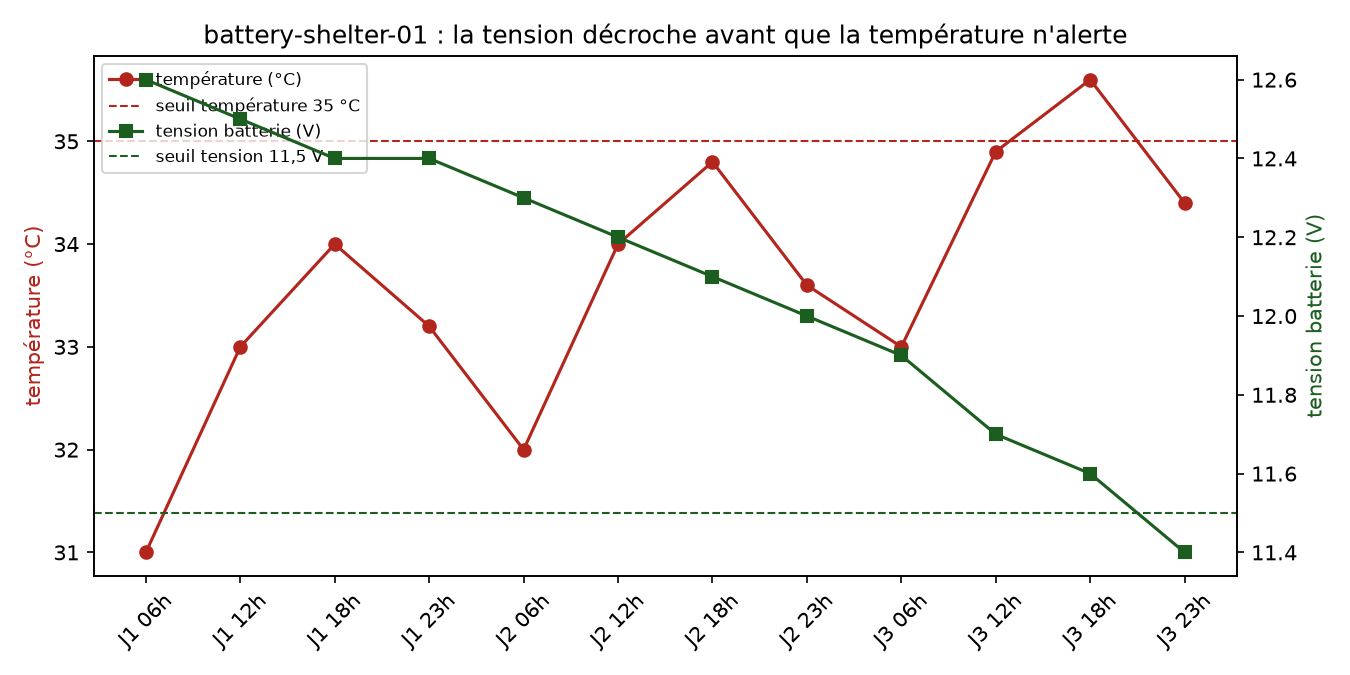
\includegraphics[width=.85\textwidth]{battery_divergence.png}
\end{frame}

\begin{frame}{Ce que le graphique révèle}
  La tension de \texttt{battery-shelter-01} décroît de façon quasi continue, de 12,6\,V à 11,4\,V, dès le premier jour.
  \begin{alertblock}{Deux signaux, deux histoires}
    La température ne franchit son seuil qu'au tout dernier point observé (35,6\,°C, 11 novembre 18h). La tension franchit le sien (\texttt{<= 11,5\,V}) seulement à la toute dernière mesure -- mais sa tendance à la baisse était visible dès le début.
  \end{alertblock}
  \normalsize Le signal précoce n'était pas celui qu'on regardait en premier.
\end{frame}

\begin{frame}{Auto-vérification avant de continuer}
  \small
  \begin{block}{Lequel des deux signaux aurait permis d'agir le plus tôt ?}
    La tension : sa tendance à la baisse est nette dès le premier jour, bien avant toute alerte de température.
  \end{block}
  \begin{block}{Un filtre unique à 35\,°C aurait-il permis de voir ce que révèle le graphique combiné ?}
    Non : un tel filtre ne concerne que la température ; il n'aurait rien montré de la tension avant le tout dernier point.
  \end{block}
\end{frame}

\begin{frame}[plain]
  \centering
  \Huge Section 4\\[3mm]
  \Large Incident : fuel-storage-01
  \vfill
  \normalsize Une zone déjà connue depuis la séquence 5, désormais surveillée en continu.
\end{frame}

\begin{frame}{Incident -- une zone sous surveillance depuis la séquence 5}
  \large \texttt{fuel-storage-01} est surveillée depuis l'incident de la séquence 5. Son seuil réel de 28\,°C est documenté dans la feuille Seuils depuis le début de la séance.
  \decisionquestion{Votre colonne alerte, construite au TP 2, avait-elle déjà cette zone sous les yeux ?}
\end{frame}

\begin{frame}{Le graphique}
  \centering
  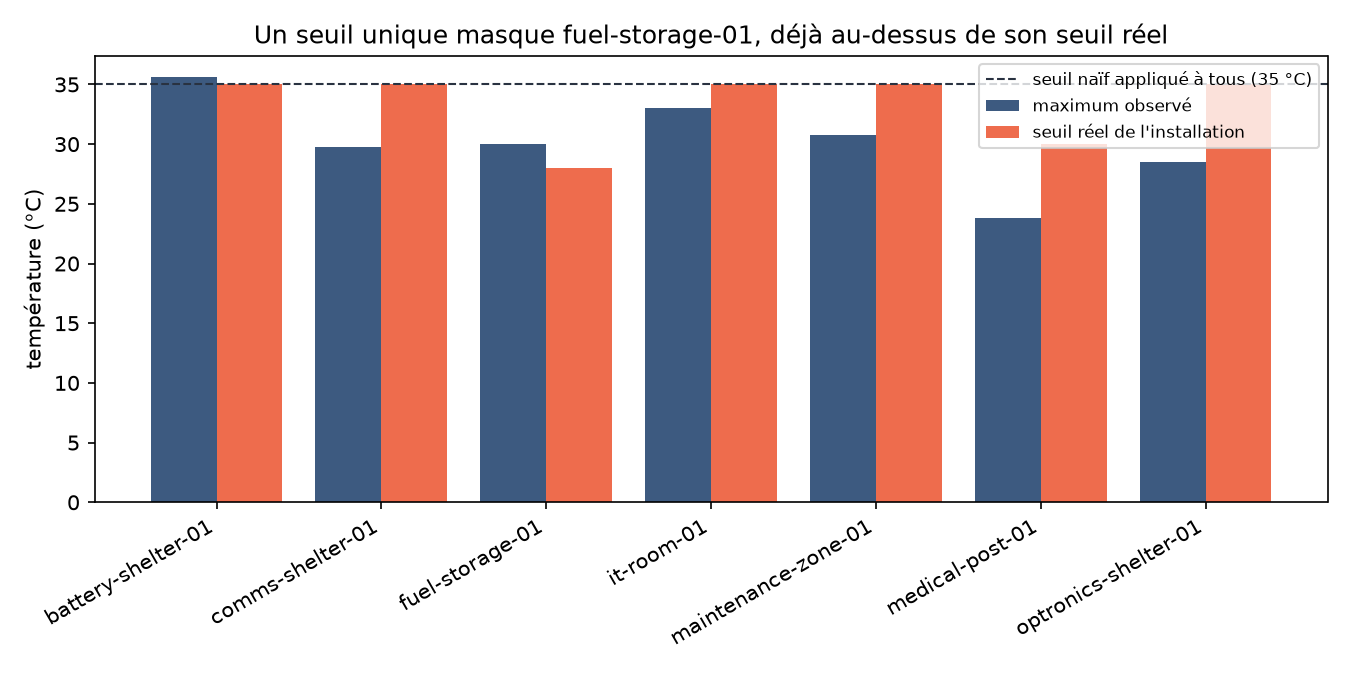
\includegraphics[width=.85\textwidth]{threshold_comparison.png}
\end{frame}

\begin{frame}{Ce que le seuil unique n'a jamais pu voir}
  \texttt{fuel-storage-01} reste entre 28,4 et 30,0\,°C sur les trois jours : jamais proche du seuil pédagogique unique de 35\,°C utilisé pour les autres zones.
  \begin{alertblock}{Le fait opérationnel manquant}
    Un dépôt de carburant a un seuil de sécurité réel bien plus bas, en raison du risque de vapeurs inflammables -- déjà établi en séquence 5. Sur les douze mesures du lot, sans exception, la zone dépasse ce seuil réel de 28\,°C.
  \end{alertblock}
  \normalsize Un seuil unique, même raisonnable pour la majorité des zones, ne peut par construction jamais détecter une installation dont le seuil réel est différent -- ici, plus sévère, jamais atteint par le seuil commun.
\end{frame}

\begin{frame}{Auto-vérification avant de continuer}
  \small
  \begin{block}{Ce résultat était-il visible dans le TCD du TP 1 ?}
    Non : ce TCD ne comparait à aucun seuil. Même en gardant 35\,°C à l'esprit, aucune valeur de \texttt{fuel-storage-01} ne s'en approche.
  \end{block}
  \begin{block}{fuel-storage-01 a-t-elle le même comportement que battery-shelter-01 ?}
    Non : l'une dérive progressivement vers un seuil commun, l'autre est stable mais au-dessus d'un seuil plus sévère, propre à elle, depuis la première mesure.
  \end{block}
\end{frame}

\begin{frame}[plain]
  \centering
  \Huge Section 5\\[3mm]
  \Large Décider
  \vfill
  \normalsize Nous revenons à la question du début de journée, avec deux zones diagnostiquées.
\end{frame}

\begin{frame}{Décision -- zones à vérifier en priorité}
  \begin{block}{Consigne}
    Remplir la feuille Note de décision du classeur.
  \end{block}
  \begin{enumerate}
    \item quelles zones vérifier en priorité, et pourquoi ces deux-là précisément ;
    \item les cinq autres zones sont-elles à ignorer pour autant ;
    \item quel onglet, quel TCD ou quelle colonne cite votre preuve ;
    \item quelle vérification terrain proposer en priorité.
  \end{enumerate}
  \alert{Une vérification uniforme sur toutes les zones n'est pas une réponse acceptable : la note doit distinguer explicitement les deux zones surveillées des cinq zones calmes.}
\end{frame}

\begin{frame}{Ce qu'aucun seuil unique ne peut faire}
  \begin{block}{Le seuil unique, seul}
    Ne peut pas signaler une installation dont le seuil réel diffère de celui appliqué à toute la base.
  \end{block}
  \begin{block}{La moyenne sur plusieurs jours, seule}
    Ne peut pas signaler une dérive progressive qui ne franchit un seuil qu'en toute fin de période.
  \end{block}
  \begin{alertblock}{Ce qui reste nécessaire dans les deux cas}
    Une recherche de seuil propre à chaque type d'installation, et une décomposition temporelle avant de conclure sur une moyenne globale.
  \end{alertblock}
\end{frame}

\begin{frame}{Transition vers la suite du cours}
  La prochaine séquence s'appuie directement sur ce classeur :
  \begin{enumerate}
    \item construire, à partir des mêmes indicateurs, un tableau de bord Excel lisible pour un décideur pressé ;
    \item choisir des graphiques qui n'exagèrent pas la certitude, comme en séquence 6 ;
    \item défendre à l'oral une recommandation sur les zones à surveiller.
  \end{enumerate}
  \vfill
  Retenez ce réflexe : avant tout agrégat, vérifier que la colonne agrégée ne contient qu'une seule grandeur, et que le seuil utilisé est bien celui de l'installation concernée.
\end{frame}

\begin{frame}{Activité -- Synthèse individuelle}
  Complétez les trois phrases, seul et sans échanger :
  \begin{enumerate}
    \item Un agrégat Excel permet d'affirmer que ...
    \item Il ne permet pas d'affirmer que ...
    \item Avant de présenter un indicateur Excel, je vérifierais ...
  \end{enumerate}
  \vfill
  \alert{Moyenne mélangée $\rightarrow$ filtrage par capteur $\rightarrow$ TCD par jour $\rightarrow$ seuil par installation $\rightarrow$ décision différenciée.}
\end{frame}

\begin{frame}{Ce que la séance a permis d'établir -- synthèse de référence}
  \small
  \begin{block}{Résultat de référence sur ce lot}
    Moyenne brute 24,05 (sans sens, quatre grandeurs mélangées). Moyenne filtrée de \texttt{battery-shelter-01} 33,62\,°C, masquant un maximum de 35,6\,°C le troisième jour. Tension de cette même zone en baisse continue de 12,6 à 11,4\,V. \texttt{fuel-storage-01} en permanence au-dessus de son seuil réel de 28\,°C, jamais proche du seuil unique de 35\,°C.
  \end{block}
  \begin{block}{Une recommandation défendable, à titre d'exemple}
    Vérifier en priorité \texttt{battery-shelter-01} (tension) et \texttt{fuel-storage-01} (seuil propre à l'installation) ; confiance moyenne sur ces deux zones, faible sur toute conclusion s'appuyant sur un seuil unique appliqué à toute la base.
  \end{block}
  \normalsize
  \alert{D'autres formulations restent recevables si elles distinguent explicitement le piège du mélange de grandeurs de celui du seuil unique, et citent une preuve précise pour chaque zone signalée.}
\end{frame}

\begin{frame}{Références et ressources}
  \tiny
  \begin{itemize}
    \item Microsoft, documentation RECHERCHEX (XLOOKUP) : \url{https://support.microsoft.com/fr-fr/office/fonction-recherchex-91f4b70a-d5b0-4b48-b81e-e0af7cae8ed7}
    \item Microsoft, créer un tableau croisé dynamique pour analyser des données : \url{https://support.microsoft.com/fr-fr/office/cr%C3%A9er-un-tableau-crois%C3%A9-dynamique-pour-analyser-des-donn%C3%A9es-de-feuille-de-calcul-a9a84538-bfe9-40a9-a8e9-f99134456576}
    \item Tukey, J. W., \emph{Exploratory Data Analysis}, 1977 -- sur les limites des résumés statistiques uniques.
    \item NIST/SEMATECH, \emph{e-Handbook of Statistical Methods} : \url{https://www.itl.nist.gov/div898/handbook/}
    \item Microsoft, appliquer une mise en forme conditionnelle : \url{https://support.microsoft.com/fr-fr/office/utiliser-la-mise-en-forme-conditionnelle-pour-mettre-en-%C3%A9vidence-des-informations-fffab983-6ce0-4188-9d15-5b422b7fe5e2}
  \end{itemize}
\end{frame}

\end{document}
